\section{{(old)Results in 8-node cluster}}
\subsection{Setup}

We set up Yarn with \name on a cluster having 8 worker nodes on CloudLab. Totally, the cluster has 256 cpu cores, and 256 GB memory.

Yarn setting. 

We use the Facebook workload traces from SWIM \cite{SWIM} for batch jobs while interactive jobs are separately created. The SWIM workload include the MapReduce jobs to simulate the real workload in from a Facebook data center for 600 servers. However, SWIM workload does not have the information of demand on each resource dimension.  We generate the CPU and MEMORY demands as in Figure 1 of \cite{drf}. The batch jobs are CPU bound jobs. There CPU demand of a batch job is from 1 to 7 cpus while it mainly requires from 3GB to 4GB memory. 

%\todo{Need to choose the number of maps, and reduces as SWIM use the same number of maps and reduces for all jobs.}

\diff{We emulate the jobs using the BigBend workload traces. The details of resource usage are in Figure \ref{fig:b3_res_usage_SpeedFair_BB}. From the traces, we create the jobs that have the same structures, resource demand, and task durations. The jobs are encoded using TEZ and submitted to YARN for scheduling.}

\textbf{Bursty users' inputs}. To guarantee the bursty users' inputs, we first compute resource rate and duration that they require. We run only interactive jobs to estimate the completion time, and the average demand of them.
\begin{itemize}
	\item bursty jobs arrive in every 100 secs.
	\item On average, a bursty job having 2 phases (map and reduce) takes 30 secs to complete. As most of resources are used in the Map phase, we set the stage 1 duration at 20 secs as it requires a lot of resources for the first 20 secs for the map tasks. The resource rate for the stage 1 is 100\% of the cluster (256 GB, 256 vcores).
\end{itemize}

\textbf{Batch jobs queues.} All batch jobs are submitted at time $t=0$.

\subsection{resource usage in details}

\begin{figure}
\centering
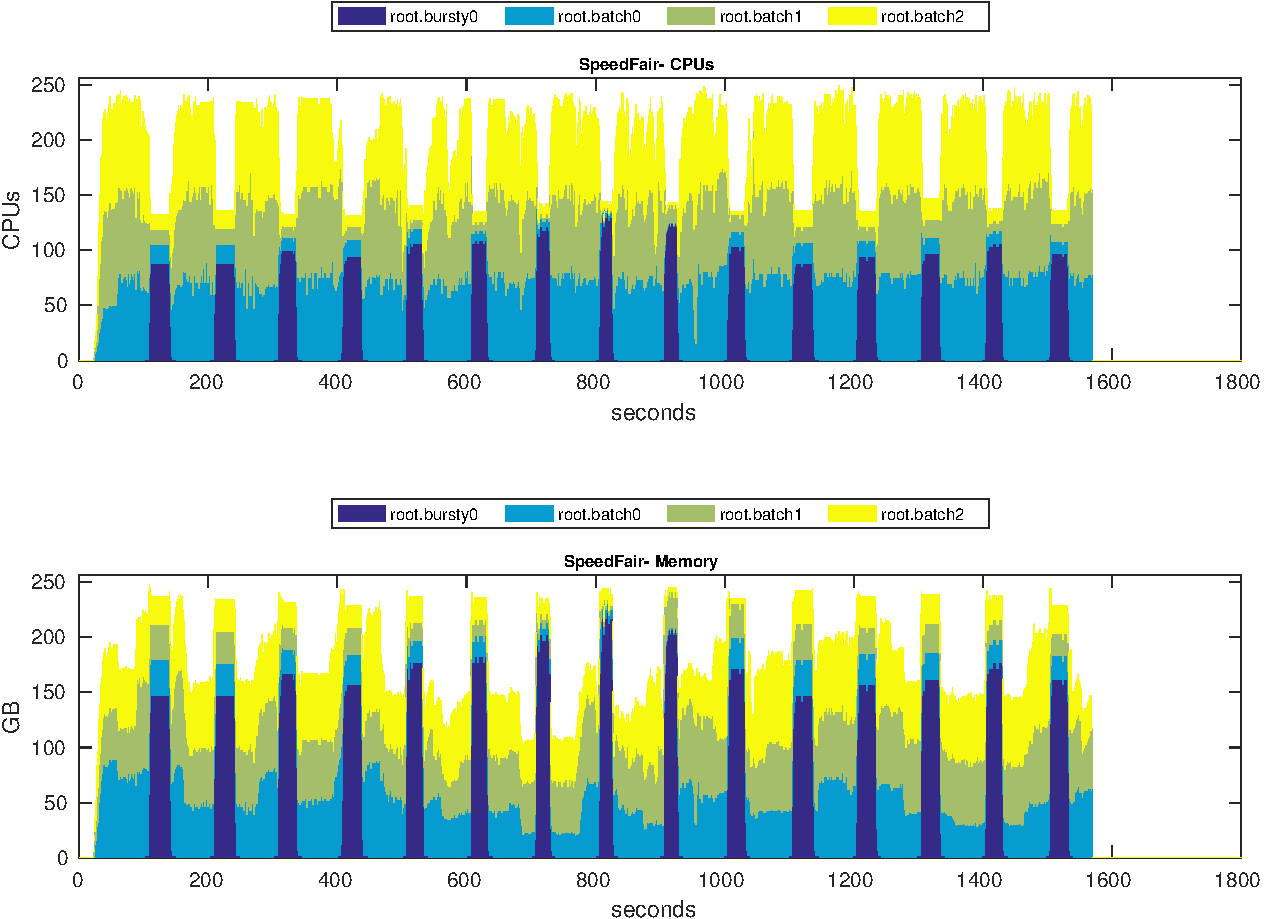
\includegraphics[width=1.0\linewidth]{fig/swim_b3_res_usage_SpeedFair}
\caption{\textbf{Workload: SWIM (FB MapReduce)} \diff{Resource usage of using SpeedFair. There are 2 unexpected points in this figures: The overall resource utlization is a bit low and SpeedFair should have more resource. The resource utilization is a bit low because all batch jobs in a queue is scheduled in a FIFO manner so there are at most 4 jobs can run at the same time. Furthermore, every job requires a lot of resources in Map phase but very litte in Reduce phase. SpeedFair cannot be allocated more resources because of non-preemption. Please compare with the Strict method in Figure \ref{fig:swim_b3_res_usage_strict} for its correctness. } }
\label{fig:swim_b3_res_usage_SpeedFair}
\end{figure}

\begin{figure}
\centering
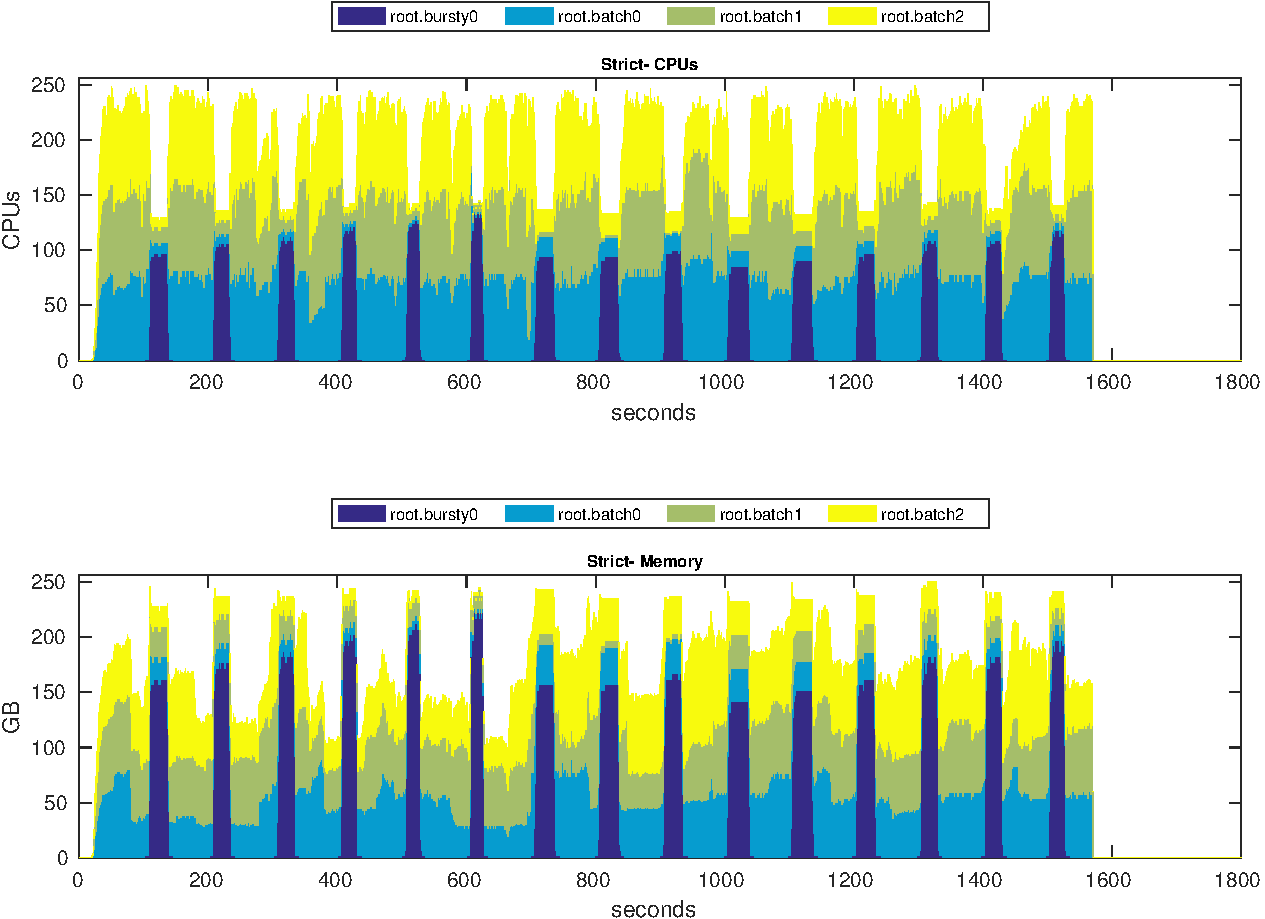
\includegraphics[width=1.0\linewidth]{fig/swim_b3_res_usage_Strict}
\caption{\textbf{Workload: SWIM (FB MapReduce)} \diff{Resource usage of using Strict. Strict actually uses DRF with a very high weight for the bursty queue. The weight of the root.bursty0 queue is set at 999999.}}
\label{fig:swim_b3_res_usage_Strict}
\end{figure}


\begin{figure}
\centering
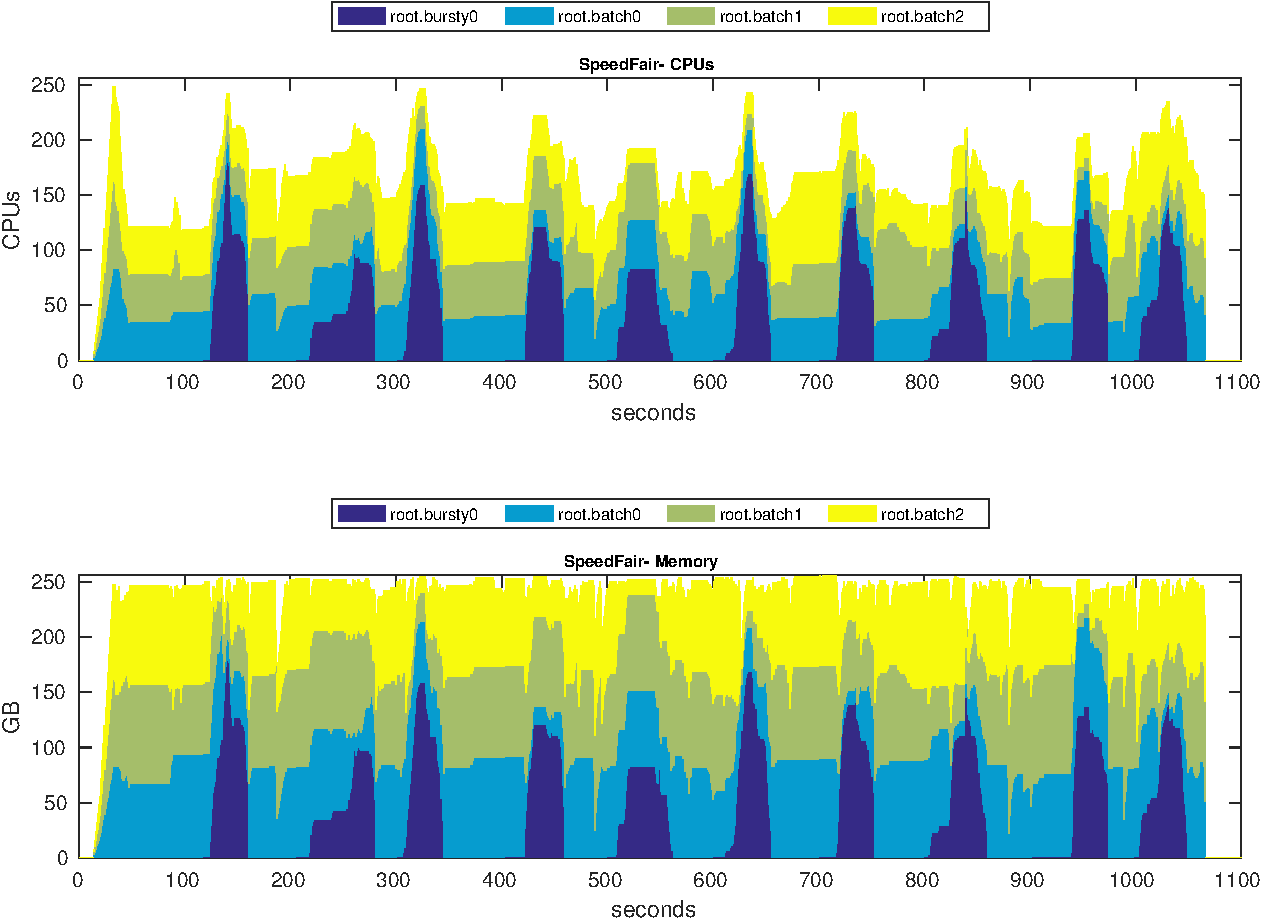
\includegraphics[width=1.0\linewidth]{fig/b3_res_usage_SpeedFair_BB}
\caption{\diff{\textbf{Workload: BigBench (Tez). SpeedFair.} The resource usage of bursty jobs are not as high as in the simulation. What are the reasons behind this? Some reasons could be: non-preemption and slow start of tasks.}}
\label{fig:b3_res_usage_SpeedFair_BB}
\end{figure}

\begin{figure}
\centering
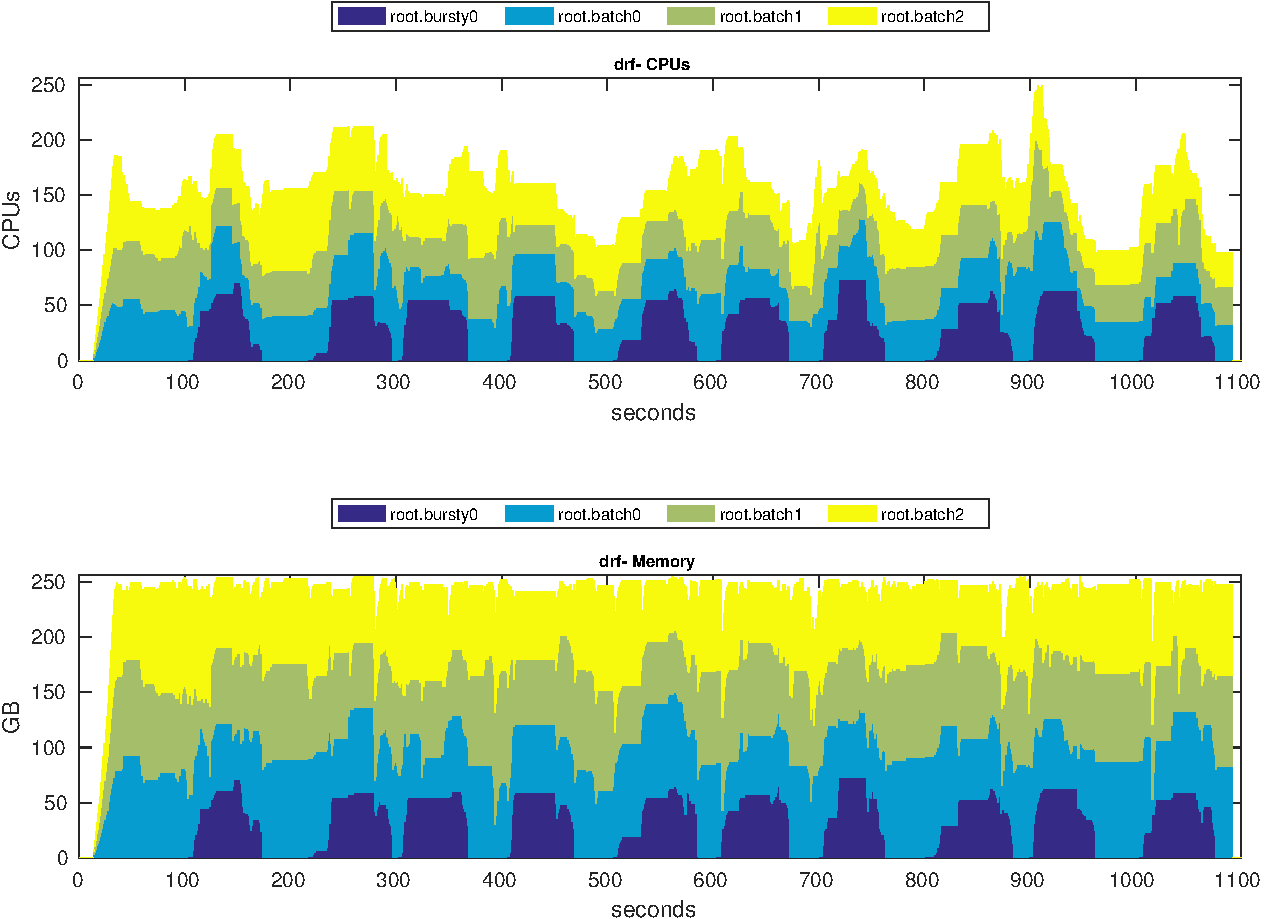
\includegraphics[width=1.0\linewidth]{fig/b3_res_usage_drf_BB}
\caption{\diff{\textbf{Workload: BigBench (Tez). DRF.} }}
\label{fig:b3_res_usage_drf_BB}
\end{figure}

\begin{figure}
\centering
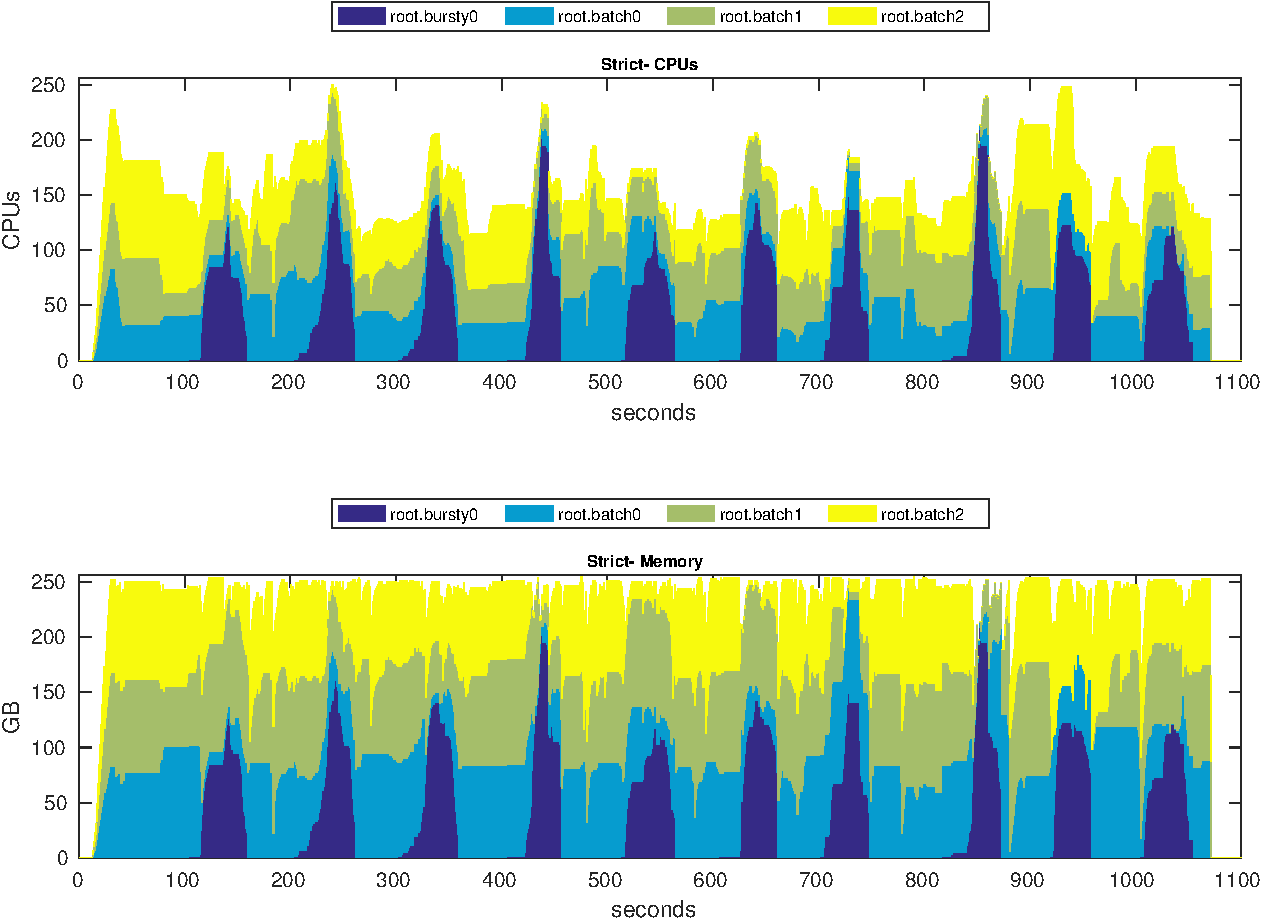
\includegraphics[width=1.0\linewidth]{fig/b3_res_usage_Strict_BB}
\caption{\diff{\textbf{Workload: BigBench (Tez). Strict}}}
\label{fig:b3_res_usage_Strict_BB}
\end{figure}


\subsection{Bursty Regular jobs}

Figure \ref{fig:exp_interactive_compl_time} shows that \textbf{the completion time of jobs are not changed} when having more queues.

\begin{itemize}
	\item Graph type: bar chart.
	\item X-axis: Number of batch queues (1, 2, 4, 8).
	\item Y-axis: Completion time.
\end{itemize}

%\begin{figure}
%\centering
%\includegraphics[width=1.0\linewidth]{fig/exp_interactive_compl_time}
%\caption{(Old figure) Need to be updated}
%\label{fig:exp_interactive_compl_time}
%\end{figure}

\subsection{Bursty jobs with variant resource demand}

\textbf{Figure}: Interactive Job completion time for variant bursty jobs (optional)
\begin{itemize}
	\item Graph type: bar chart.
	\item X-axis: Number of batch queues (1, 3, 5, 8).
	\item Y-axis: Completion time.
\end{itemize}

\textbf{Figure}: Snapshot of Multiple Resource Allocation on Memory  Figure \ref{fig:res_usage_speedfair_exp}

%\begin{figure*}[!t]
%	\centering
%	\subfloat[DRF]{\includegraphics[width=1.0\linewidth]{fig/drf-vcore_usage}}
%	\\
%	\subfloat[SpeedFair]{\includegraphics[width=1.0\linewidth]{fig/SpeedFair-ram_usage}}
%	\caption{Resource Allocation in CPU (vcores)}
%	\label{fig:res_usage_speedfair_exp}2.5
%\end{figure*}

%\begin{figure*}[!t]
%	\centering
%	\subfloat[DRF]{\includegraphics[width=1.0\linewidth]{fig/drf-vcore_usage}}
%	\\
%	\subfloat[SpeedFair]{\includegraphics[width=1.0\linewidth]{fig/SpeedFair-ram_usage}}
%	\caption{Resource Allocation on Memory}
%	\label{fig:res_usage_speedfair_exp}
%\end{figure*}


\section{More Figures in details to debug}

What are the gaps between simulation and experiment.

\subsection{is slow-start the problem?}
\todo{Plot only bursty jobs to see what happens.}
\begin{figure}
\centering
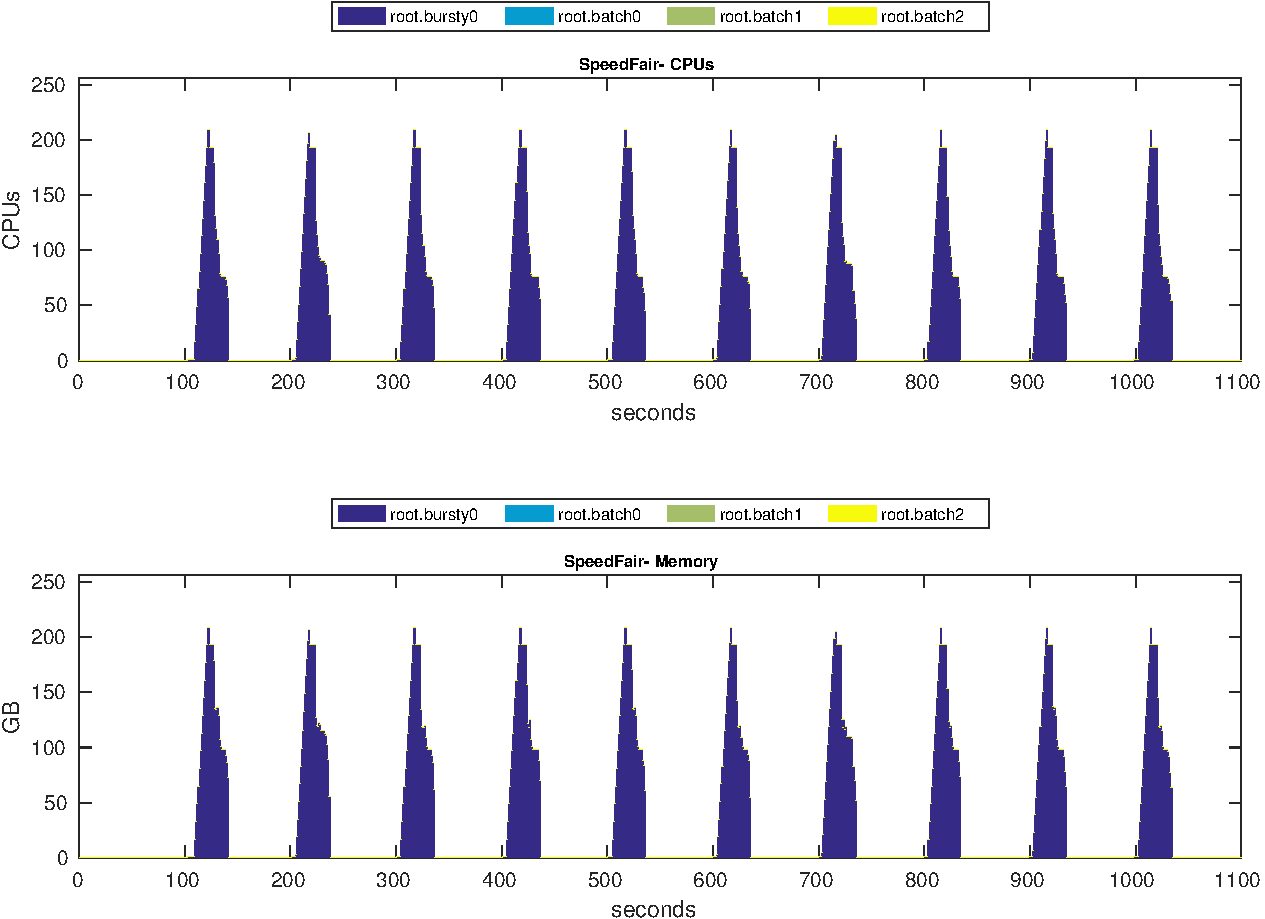
\includegraphics[width=1.0\linewidth]{fig/b3_res_usage_SpeedFair_BB_bursty}
\caption{\diff{\textbf{Ony busry jobs. Workload : BigBench (TEZ).} } We can see the job is allocated resource slowly. We call this phenomenon ``slow start" }
\label{fig:b3_res_usage_SpeedFair_BB_only}
\end{figure}

\subsection{is non-preemption the problem?}
\todo{Use the short bursty jobs and batch jobs, to see what happen.}

\begin{figure}
\centering
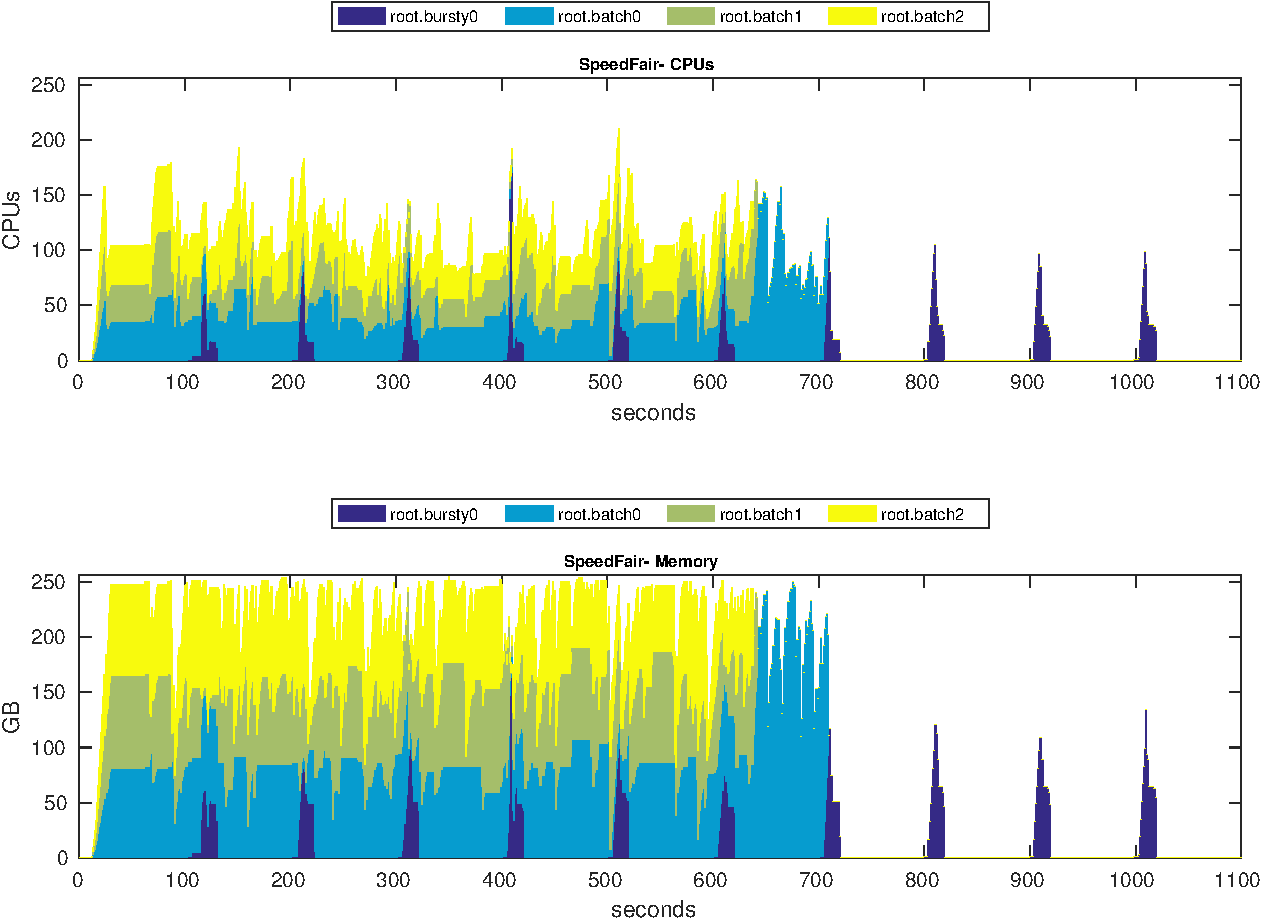
\includegraphics[width=1.0\linewidth]{fig/b3_res_usage_SpeedFair_BB_1s}
\caption{\diff{\textbf{Uniform Workload (1 sec per task): BigBench (TEZ). SpeedFair}.} Since the task is too short and the tasks in the same stage do not start at the same time (\textbf{slow start}), the bursty jobs do not need the full capacity.}
\label{fig:b3_res_usage_SpeedFair_BB_1s}
\end{figure}

\begin{figure}
\centering
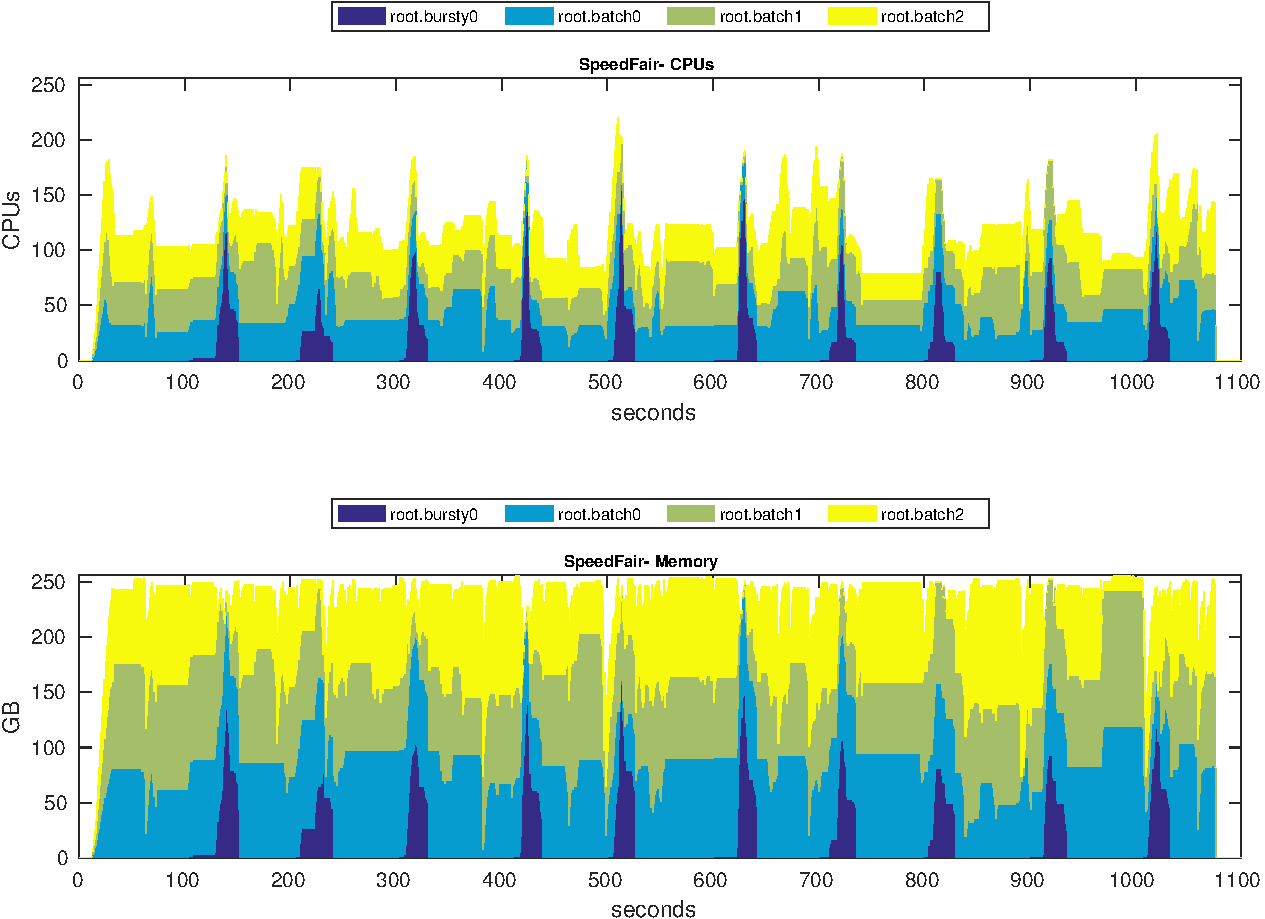
\includegraphics[width=1.0\linewidth]{fig/b3_res_usage_SpeedFair_BB_3s}
\caption{\diff{\textbf{Uniform Workload (3 sec per task): BigBench (TEZ). SpeedFair. This may have the same slow start prolem like 1sec uniform workload. However, we can see some impact from non-preemtion at 100, 600, ...} }}
\label{fig:b3_res_usage_SpeedFair_BB_3s}
\end{figure}

\begin{figure}
\centering
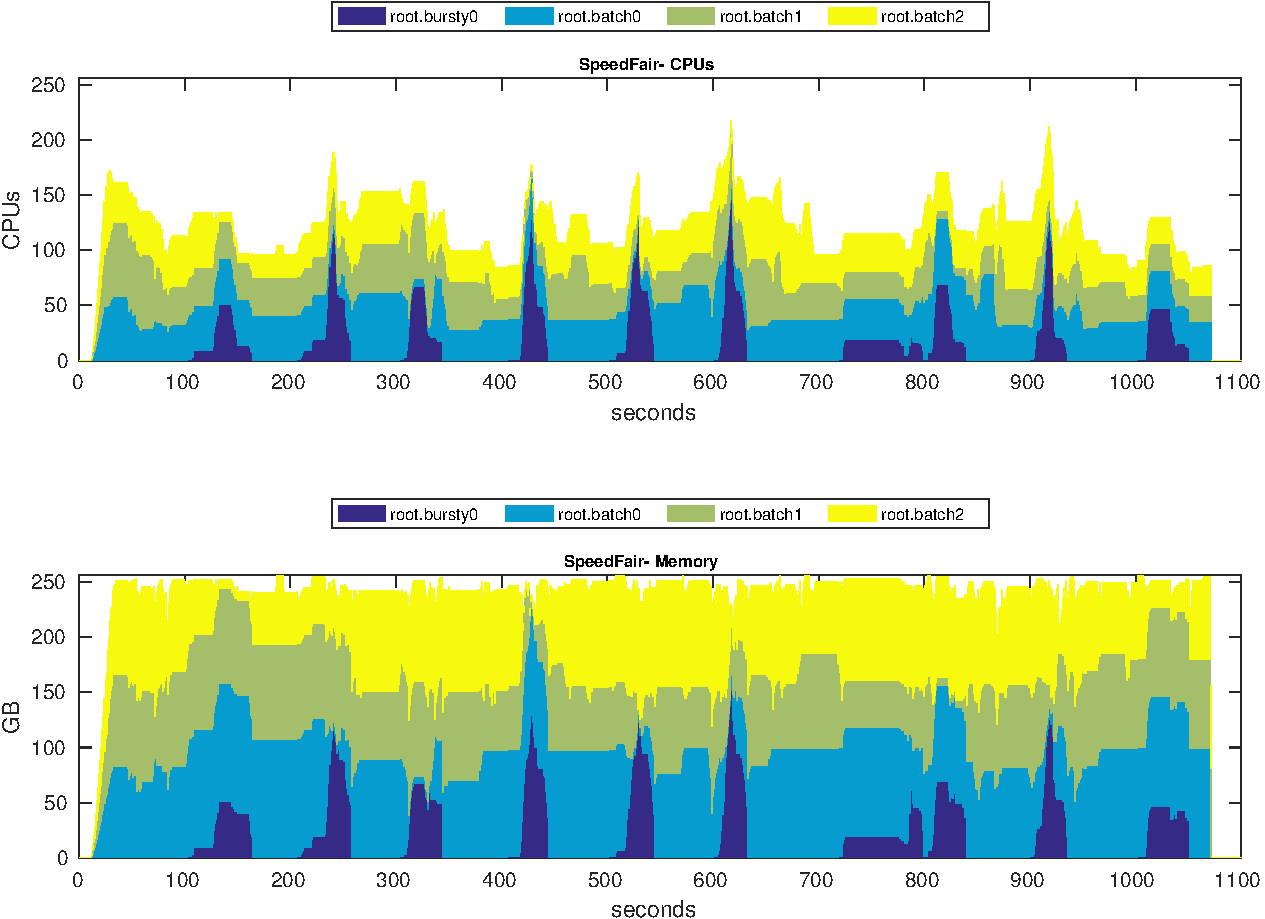
\includegraphics[width=1.0\linewidth]{fig/b3_res_usage_SpeedFair_BB_5s}
\caption{\diff{\textbf{Uniform Workload (5 sec per task): BigBench (TEZ).} }}
\label{fig:b3_res_usage_SpeedFair_BB_3s}
\end{figure}

\subsection{What else? May be Tez Scheduler?}



\newpage

\section{Work on the non-preemption and slow start issues}

\subsection{Enable preemption in Yarn}

We enable preemption in Yarn in Figure \ref{fig:b3_res_usage_SpeedFair_BB_preemption}. It has the same job profiles of Figure \ref{fig:b3_res_usage_SpeedFair_BB}. However, there is no significant improvement. The reasons may be: (1) \textbf{preempting a containter (for a task) is too slow}, (2) \textbf{allocating a containter (for a task) is too slow}. (1) is not the root cause as we already set preemption timeout at 100 ms, which kills a container to release the resource roughly in 100 ms. So, the speed of preemption is negligible. The slowly allocating a container for each task must be the problem here.


\begin{figure}
\centering
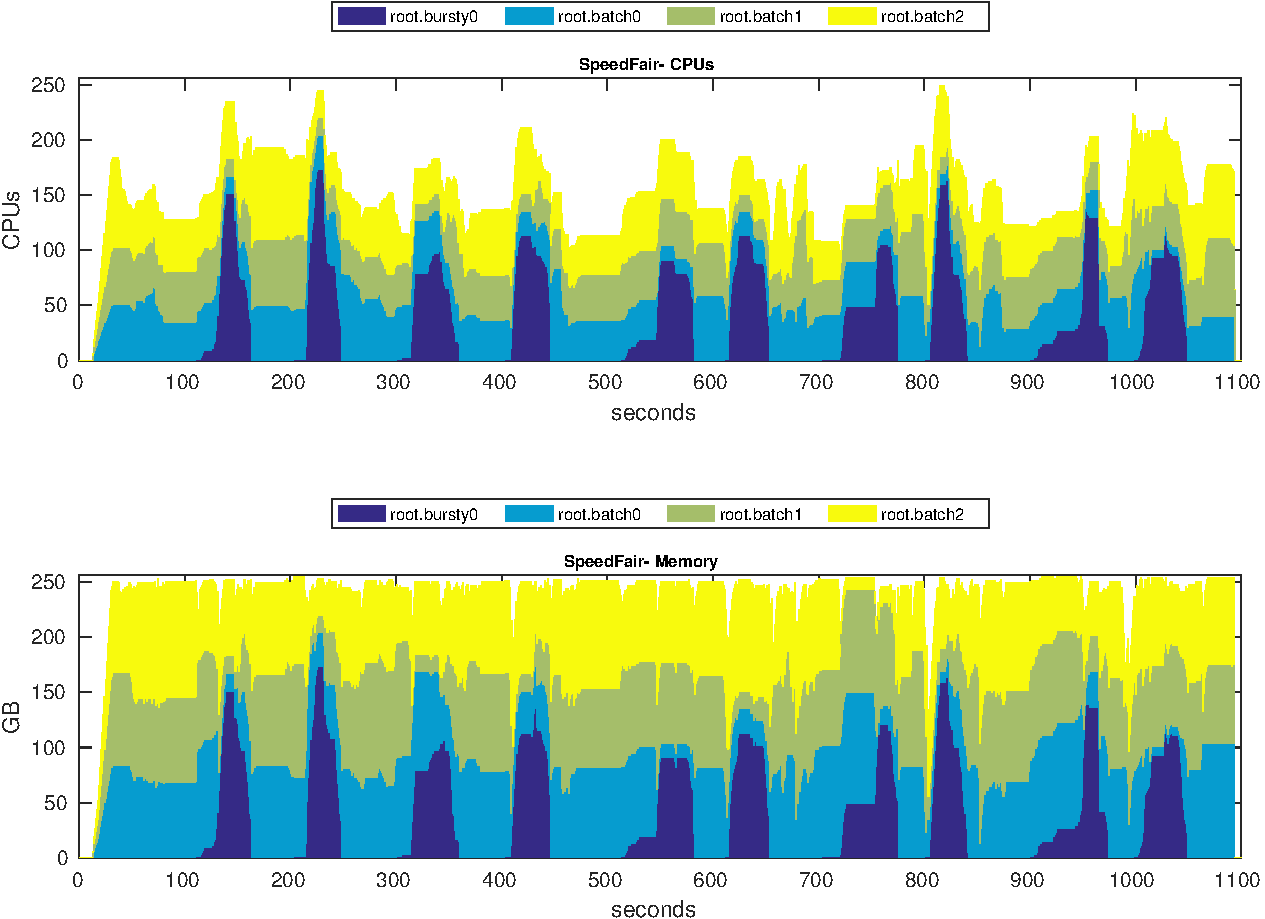
\includegraphics[width=1.0\linewidth]{fig/b3_res_usage_SpeedFair_BB_preemption}
\caption{\diff{\textbf{Preemption is ENABLED.} Workload: BigBench (TEZ).} Although the preemption is enabled, it is is not close to Figure \ref{fig:b3_res_usage_SpeedFair_BB_only}, it is NOT much better than Figure \ref{fig:b3_res_usage_SpeedFair_BB}.}
\label{fig:b3_res_usage_SpeedFair_BB_preemption}
\end{figure}

\textbf{Slowly allocating a container:} To confirm this, we run increase the duration of the every job of the bursty jobs 5x times. The results is detailed in Figure \ref{fig:b3_res_usage_SpeedFair_BB_5x}. Preemption helps the long-task duration bursty jobs here. In fact, the slowly allocating a container is  is related to the ``slow start'' issue.

\begin{figure}
\centering
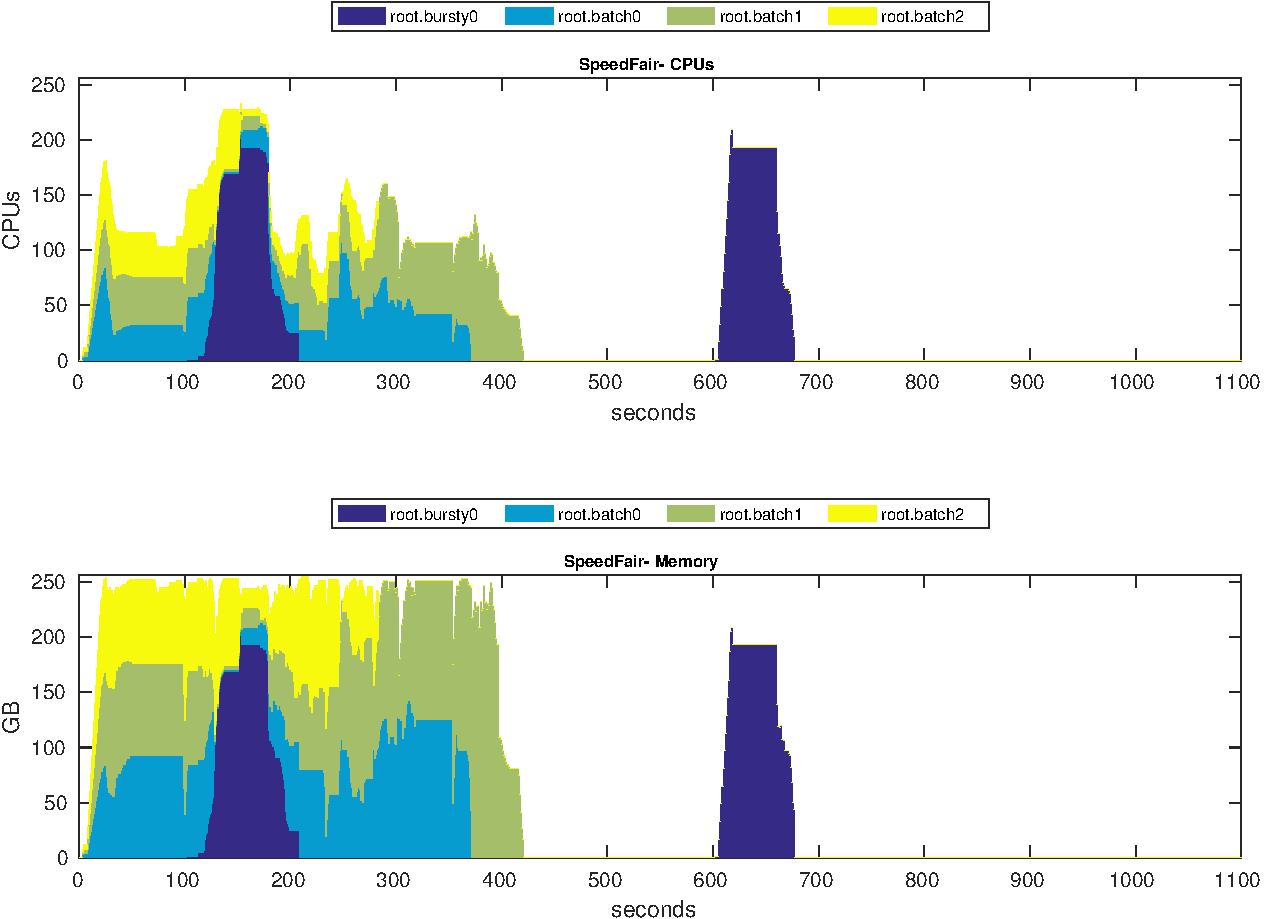
\includegraphics[width=1.0\linewidth]{fig/b3_res_usage_SpeedFair_BB_5x}
\caption{\diff{\textbf{Preemption is ENABLED, task duration 5x.} Workload: BigBench (TEZ).} The preemption help bursty jobs when the task duration is much longer.}
\label{fig:b3_res_usage_SpeedFair_BB_5x}
\end{figure}


\subsection{Slow Start in Yarn}

The slow start issue is clearly shown in Figure \ref{fig:b3_res_usage_SpeedFair_BB_only}. When we run only a bursty job in the cluster, it takes 20 secs to reach the peak demand. In the first few seconds (7 secs in the figure), every job needs a single container (e.g., 1 cpu 1GB ram) for its application master (AM) (We can see when zoom the figure in.). This AM does the setup process in 7 secs but it is unavoidable. When the AM requests more resources, the demand is increasing reach to the peak demand next 13 secs (because the task duration of the first stage is 13 secs.). The similar slow start happens for the second bursty job in figure \ref{fig:b3_res_usage_SpeedFair_BB_5x}.

What is the root cause of slow start? The reason behind is that Yarn allocates the container (for a task) one by one to a single job. If the number of tasks is large, the slow start will have more negative impact on on our approach. Yarn has to allocate a container one by one to maintain the consistency of cluster distributed resources for multiple requests.

We implement the simulator for the larger clusters with larger workload.

\begin{itemize}
	\item DRF: 
	\item DRF-W: The weight of the interactive queue is set at 4.0 while others are 1.0.
	\item Strict Priority: Strict Priority is basically DRF-W in which the bursty queues have very high weights (e.g. positive infinity).
\end{itemize}


\noindent \textbf{Metrics:} Average completion time

\begin{itemize}
	\item How much does our proposed policy improve the performance?
\end{itemize}

\subsection{Job completion time improvement for short bursty jobs }


We run our algorithm and other baseline methods on 1 single bursty queue and a number of batch queues.

Figure \ref{fig:BB-compl_time} show the results of using Big bench workload. X-axis show the number of batch queues.
\begin{itemize}
\item The completion time of busty jobs are guaranteed as same as Strict's when the number of queues increases from 1 to 4. When the number of batch queues is 8, the bursty jobs cannot receive enough resources to complete in stage 1 because of non-preemption. In fact, there are many running jobs on the batch queues and we cannot just kill the running jobs to give more resources to the bursty jobs. When the number of (admitted) batch queues are more than 9, the algorithm does not admit the bursty queue.
\item The completion time of batch jobs are similar among 4 methods.
\item The completion time of batch jobs for all methods vary when we increase the number of batch queues as more batch jobs are in the cluster.
\end{itemize}

\begin{figure*}[!t]
	\centering
	\subfloat[bursty job's avg completion time]{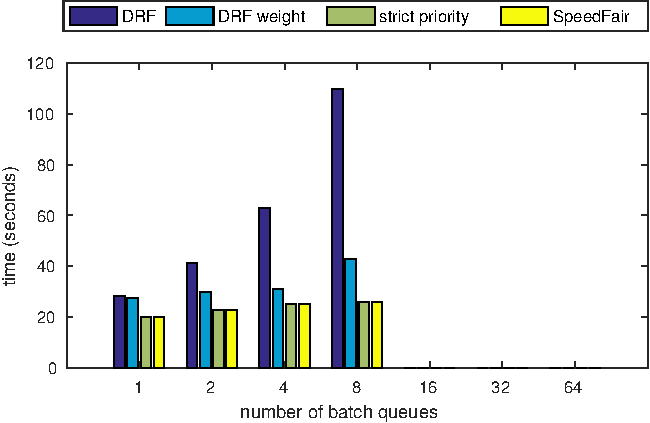
\includegraphics[width=0.3\linewidth]{fig/BB-interactive_compl_time}}
	\subfloat[batch job's avg completion time]{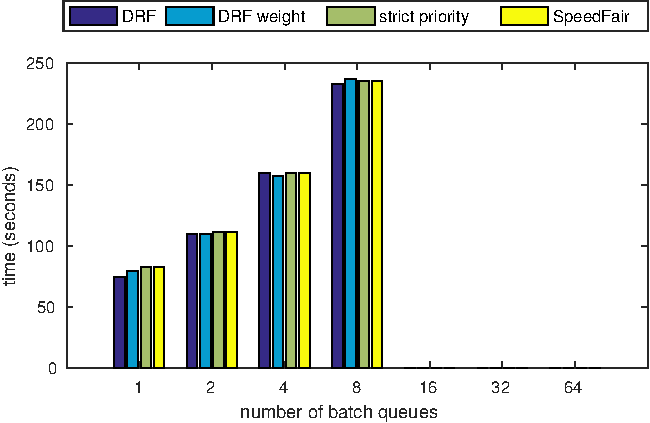
\includegraphics[width=0.3\linewidth]{fig/BB-batch_compl_time}}
	\subfloat[Histogram of task durations]{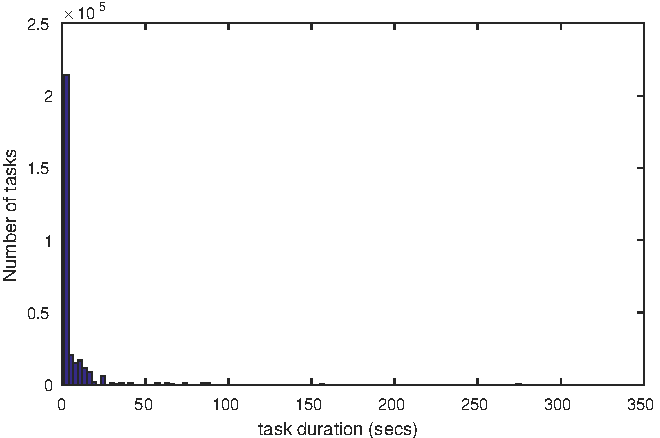
\includegraphics[width=0.3\linewidth]{fig/BB-hist}}
	\\
	\subfloat[resources usage - Speedfair]{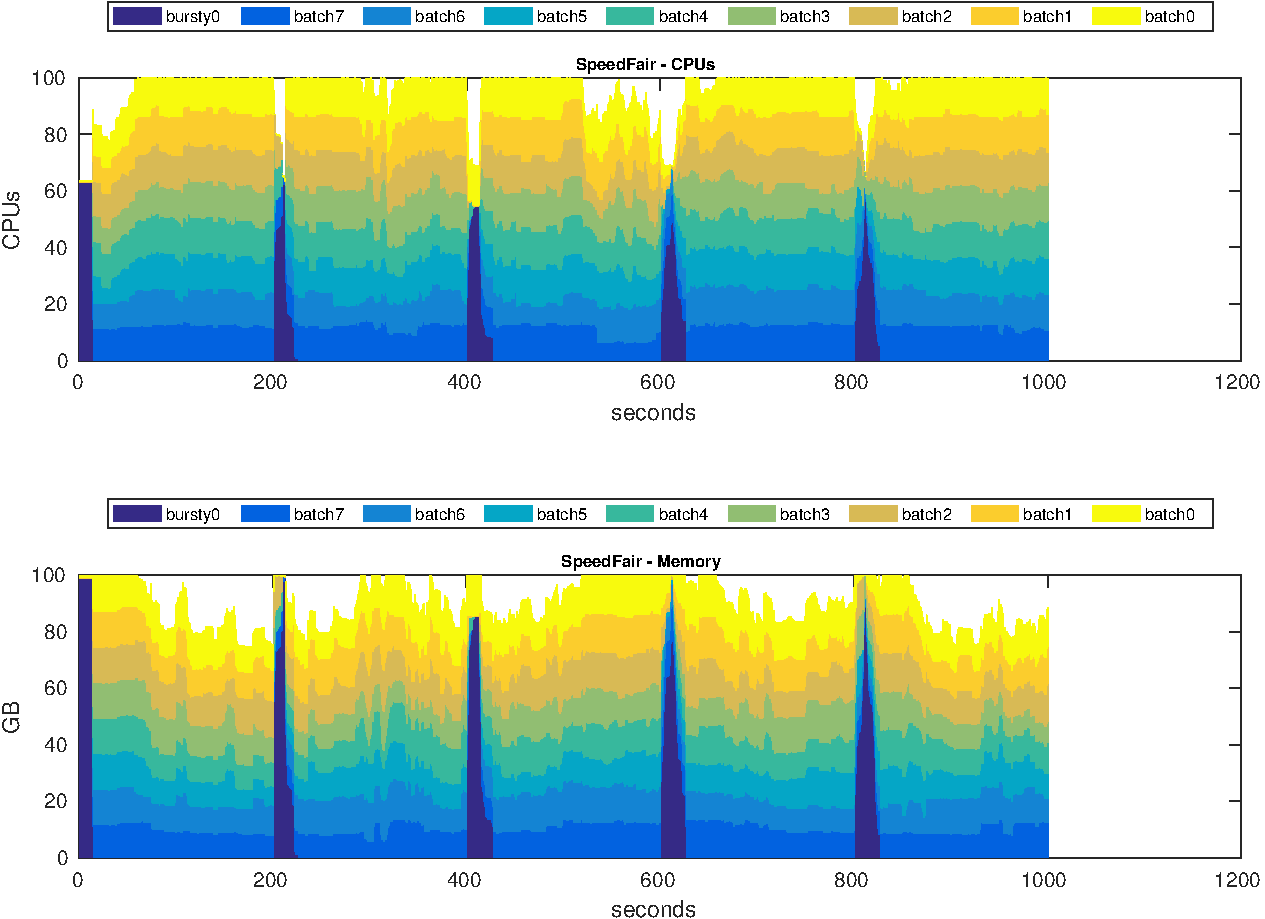
\includegraphics[width=1.0\linewidth]{fig/BB-b8_res_usage_speedfair}}
	\caption{[Simulation] Average completion time for Big Bench workload.}
	\label{fig:BB-compl_time}
\end{figure*}

Figure \ref{fig:TPC-H-compl_time} respectively show the simulation results of using TPC-H.
%\begin{itemize}
%\item Although the average bursty completion of DRF significantly increases, our method is not negatively impacted by the number of queues. The completion time is not as low as in the case of no batch queues because of non-preemption.
%\item The completion time of bursty jobs of SpeedFair are larger than Strict when the number of queues are greater than or equal to 8. The reasons behind this are non-preemption and the long task durations as in Figure \ref{fig:TPC-H-compl_time} (c). Some bursty jobs actually take longer than 50 secs to finish, which results in low resource allocation at stage 2. In the meantime, Strict asks for maximum resource any time.
%\item The completion time of batch jobs are not suffered as the batch jobs are very long.
%\end{itemize}

\begin{figure*}[!t]
	\centering
	\subfloat[bursty job's avg completion time]{
\includegraphics[width=0.3\linewidth]{fig/updated.jpg}}
	\subfloat[batch job's avg completion time]{
\includegraphics[width=0.3\linewidth]{fig/updated.jpg}}
	\subfloat[Histogram of task durations]{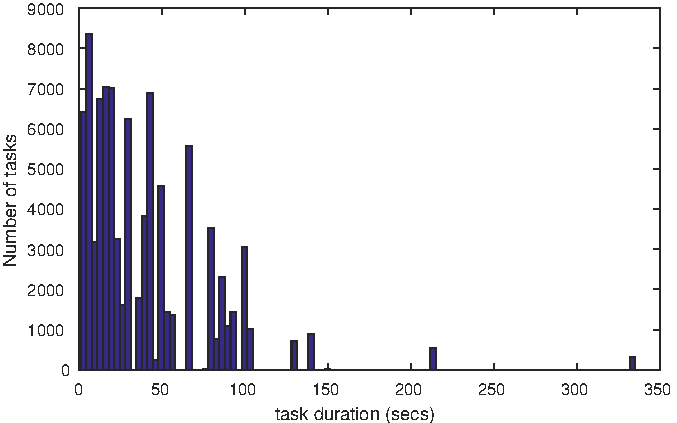
\includegraphics[width=0.3\linewidth]{fig/TPC-H-hist}}
	\caption{Average completion time for TPC-H workload.}
	\label{fig:TPC-H-compl_time}
\end{figure*}

Figure \ref{fig:TPC-DS-compl_time} show the output of running the algorithms on TPC-DS workload. The simulation results are expected for both bursty jobs and batch jobs.

\begin{figure*}[!t]
	\centering
	\subfloat[bursty job's avg completion time]{
\includegraphics[width=0.3\linewidth]{fig/updated.jpg}}
	\subfloat[batch job's avg completion time]{
\includegraphics[width=0.3\linewidth]{fig/updated.jpg}}
	\subfloat[Histogram of task durations]{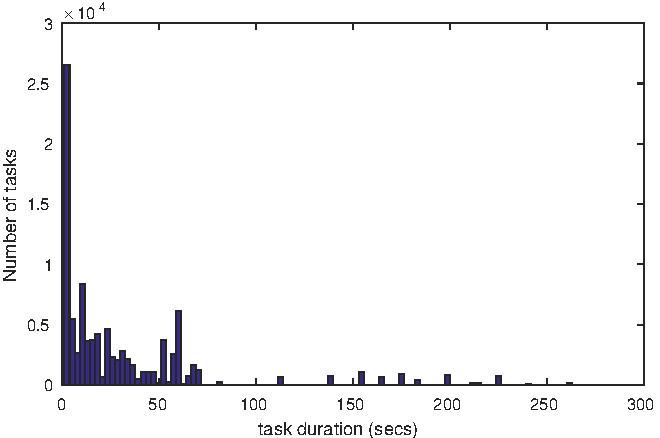
\includegraphics[width=0.3\linewidth]{fig/TPC-DS-hist}}
	\caption{Average completion time for TPC-DS workload.}
	\label{fig:TPC-DS-compl_time}
\end{figure*}

\subsection{Batch jobs completion time when running long bursty jobs}

In Figure \ref{fig:BB-scaled_bursty}, we scaled the bursty jobs from 1 to 10 and observed how they affect the batch jobs.

\begin{itemize}
\item When the users submit very long bursty jobs, the batch jobs are starved and wait for all long bursty jobs to finish.
\item In the meantime, SpeedFair prevent the problem happen and allows batch jobs get resources.
\end{itemize}

\begin{figure}
\centering
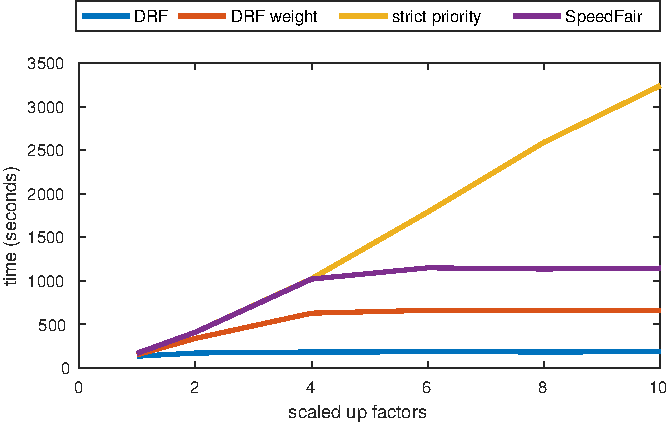
\includegraphics[width=1.0\linewidth]{fig/BB-scaled_bursty}
\caption{[Simulation] SpeedFair can prevent the batch jobs from suffering the large bursty jobs. \todo{Reduce the duration of stage 1 or increase the number of batch jobs' tasks.}}
\label{fig:BB-scaled_bursty}
\end{figure}
